\documentclass[11pt,a4paper,spanish]{book}
\usepackage{estilo_unir-1}
\hypersetup{
	colorlinks   = true, %Colours links instead of ugly boxes
	urlcolor     = blue, %Colour for external hyperlinks
	linkcolor    = black, %Colour of internal links
	citecolor   = red %Colour of citations
}



%---------------------------
%título del trabajo y autor
%---------------------------
\title{La importancia de la simetrías en física}
\author{
        \\
        \hspace{3cm}Ansony Rolando Medina Baca\\
        \hspace{3cm}Ariel Francisco Montejo Dominguez\\
       \hspace{3cm}Frank Blue Valdivia Chávez\\
      \hspace{3cm}Ruben Dario Sotelo Carrillo
        }
\date{15 de Octubre del 2024}
\profesor{Rodrigo Gil-Merino y Rubio}

%---------------------------
%marges
%---------------------------
%\usepackage[margin=1.9cm]{geometry}
%---------------------------
%---------------------------
%---------------------------
%---------------------------
\begin{document}
\renewcommand{\listfigurename}{Índice de figuras}
\renewcommand{\listtablename}{Índice de tablas}
\renewcommand{\contentsname}{Índice de contenidos}
\renewcommand{\figurename}{Figura}
\renewcommand{\tablename}{Tabla} 

\maketitle

\frontmatter
\tableofcontents
\listoffigures
\listoftables

\chapter{Resumen}
{\bf Nota:} en esta Sección se introducirá un breve resumen en español del trabajo realizado (extensión máxima: esta página). Este resumen debe incluir el objetivo o propósito de la investigación, la metodología, los resultados y las conclusiones (obviamente, todo muy resumido, pero así se sabe de un vistazo lo que se va uno a encontrar a continuación). En general, los conceptos deben estar claramente explicados (de forma resumida, repito) para que el propio resumen sea autoconsistente.\\


{\bf Palabras clave:} se deben incluir de 4 a 6 conceptos clave en español, significativos para el contenido del Trabajo (pueden ser conceptos formados por más de una palabra)

\chapter{Abstract}
{\bf Nota:} this Section should include the english version of the previous Resumen.\\


{\bf Keywords:} please include between 4 to 6 key concepts in english, relevant to the content of this report (each concept might include multiple words)

\mainmatter

\chapter{Introducción}
%En la Introducción se debe resumir de forma esquemática pero suficientemente clara lo esencial de cada una de las partes del trabajo. La lectura de esta parte debe contextualizar perfectamente todo el trabajo y debe estar PLAGADA DE REFERENCIAS.
%Es una parte muy importante de la memoria. Las ideas principales a transmitir son la identificación del problema a tratar, la justificación de su importancia, los objetivos generales a grandes rasgos y un adelanto de la contribución que esperas hacer.
%A modo de guía, la Introducción debe contener estos tres apartados:
\begin{itemize}
\item \textbf{Motivación / justificación del tema a tratar}\\
%\section{Motivación / justificación del tema a tratar}
Los principios de simetría desempeñan una función clave en la formulación de las leyes fundamentales y en el desarrollo de la física moderna. El reto al momento de describir los fenómenos físicos es abstraer las leyes subyacentes universales, a pesar de la complejidad de las condiciones iniciales, lo cual es esencial para encontrar las invariancias que permiten describir los fenómenos físicos de manera consistente\citep{gross1996}.\\
Desde la época griega, aunque no utilizaban el término "simetría", la fascinación por ella quedó plasmada en \cite{aristóteles1995}, quien escribió sobre la homogeneidad de los cuerpos, en la que todas sus partes compartían la misma naturaleza. Por otro lado, \cite{galileo1632} se refiere a la homogeneidad a nivel de la estructura del universo, donde las leyes físicas son universales y los cuerpos se comportan de manera coherente bajo las mismas reglas de movimiento. En la misma época, \cite{descartes1644} nos habla del universo como un sistema en el cual las propiedades del espacio y de la materia son uniformes y homogéneas. Descartes sería el iniciador del principio de isotropía en la física.\\
La simetría en las leyes del movimiento y de la gravitación de \cite{newton2018} se convirtió en un concepto central en la física, que contiene una noción implícita en la fuerza gravitatoria, la cual es simétrica en su dependencia radial, garantizando la coherencia y el equilibrio del sistema solar. \\
Uno de los teoremas fundamentales en la formalización de este concepto fue presentado por la matemática alemana Emmy Noether, quien, en su artículo \cite{noether1918}, a través de una rigurosa matemática, estableció la correlación entre simetría y cantidad conservada, donde las leyes de conservación (conservación de la energía, del momento angular, del momento lineal, etc.) se derivan de las propiedades de simetría de la naturaleza. La importancia de la simetría no solo ha servido de base para la física teórica, sino también para la física experimental, sirviendo de guía para la unificación de fuerzas y la predicción de nuevas partículas.\\
Por último, las invariancias encontradas nos permiten no solo distinguir los patrones regulares de los fenómenos físicos, sino que también condicionan la forma de las leyes de la naturaleza, revelando un entendimiento más profundo del universo, donde la simetría actúa como un principio organizador central.\\
\item \textbf{Planteamiento del trabajo}\\
El trabajo tiene como eje central el desarrollo de un análisis exhaustivo de la importancia de la simetría en las diferentes áreas de la física, comenzando con una revisión de sus orígenes y su evolución a lo largo del tiempo, y examinando los teoremas más relevantes que permitieron formalizar las invariancias de los fenómenos físicos. Además, durante esta revisión, se analizará la importancia de la aplicación de la simetría en la mecánica clásica, relativista y en áreas más avanzadas como la mecánica cuántica, la simetría de gauge y la ruptura de la simetría. Finalmente, se abordarán las aplicaciones recientes de las simetrías y la unificación de fuerzas. De este modo, se espera destacar la relevancia de la simetría en la formulación de las leyes físicas.\\
%\section{Planteamiento del trabajo}
\item Estructura del trabajo
%\section{Estructura del trabajo}
\end{itemize}
\vspace{2cm}
%{\bf{ATENCIÓN, CÓMO REFERENCIAR.}}

%Las referencias NO están para rellenar. Son un TRIBUTO a las personas que hicieron en primer lugar una investigación o aportaron una idea. Por tanto, se deben citar LOS TRABAJOS ORIGINALES DE LOS AUTORES, y no un libro de texto donde he visto que hablan de algo. Los libros de texto se pueden referencial excepcionalmente, porque el libro es sobresaliente y conocido en el campo y/o porque quiero apoyarme en una explicación conocida para un determinado concepto o cuestión.

%Si queremos citar a alguien, por ejemplo porque vamos a hablar de Latex \citep{lamport1994} o porque, según las ideas de \cite{ackerman2017}, la liga de fútbol inglesa debe tener torneos de desempate, pues tenemos que hacerlo correctamente, como acabamos de hacer.

%El párrafo anterior tiene dos ejemplos típicos que nos van a aparecer cuando citemos obras: la cita indirecta, cuando la ponemos entre paréntesis y la directa, cuando solo va entre paréntesis el año, pero no los autores.

%Para consultar detenidamente la formas de referenciar, debéis seguir el formato APA del siguiente documento: \url{https://bibliografiaycitas.unir.net/documentos/APA_7ed_UNIR.pdf}



\chapter{Contexto y estado de la cuestión}

En esta Sección debemos demostrar que conocemos lo que se ha hecho en el ámbito que estamos desarrollando el trabajo. En nuestro caso, que se ha buscado la bibliografía y referencias suficientes y que esas ideas se han volcado en el trabajo en la línea de los objetivos que perseguimos o que queremos transmitir.


\chapter{Objetivos}

%Esquematizar claramente los objetivos del trabajo, las ideas que queremos demostrar. Podemos tener varios tipos de objetivos. Por ejemplo, podemos tener un número de objetivos generales y otro de objetivos específicos. Deben ordenarse claramente.

\section{Objetivo general}

Establecer la importancia de la simetría en la física, analizando su impacto en la interpretación de los fenómenos naturales, así como en la predicción y la unificación de las leyes físicas.


\section{Objetivos específicos}
\begin{itemize}
\item Explorar las teorías y los conceptos de la simetría y su rol en la física clásica y moderna.
\item Analizar la relación entre la simetría y la conservación de magnitudes físicas.
\item Describir las aplicaciones de la simetría en las distintas áreas de la física, la ruptura de la simetría y las teorías de unificación de las fuerzas.
\end{itemize}    

\chapter{Desarrollo del trabajo}

Aquí desarrollaremos nuestro trabajo. Contrastaremos la ideas entre varios autores y, si es posible, con las nuestras. Podemos incluir los subapartados que necesitemos.\\

Tanto en esta Sección, como en el resto del Trabajo, se debe cuidar la redacción, el uso de las comas, puntos, puntos y coma, puntos y aparte y demás recursos. Fijaos en esta plantilla como estan escritas ciertas palabras que usamos mucho: \emph{Sección xx}, pero \emph{secciones}; \emph{Figura xx}, pero \emph{figuras}; \emph{Ecuación xx}, pero \emph{ecuaciones}; etc... Podéis echar un vistazo a trabajos de fin de estudios para comprobar la organización, ortografía y redacción de un trabajo a este nivel. En el repositorio de UNIR tenéis la posibilidad de acceder a trabajos presentados como TFMs en esta Titulación: \url{https://reunir.unir.net/handle/123456789/6218}\\

Las figuras y tablas tienen que tener su numeración y su título. Además, se debe indicar la fuente, si es de elaboración propia o se ha tomado de alguna referencia.\\

Por ejemplo:

\begin{figure}[h]
	\centerline{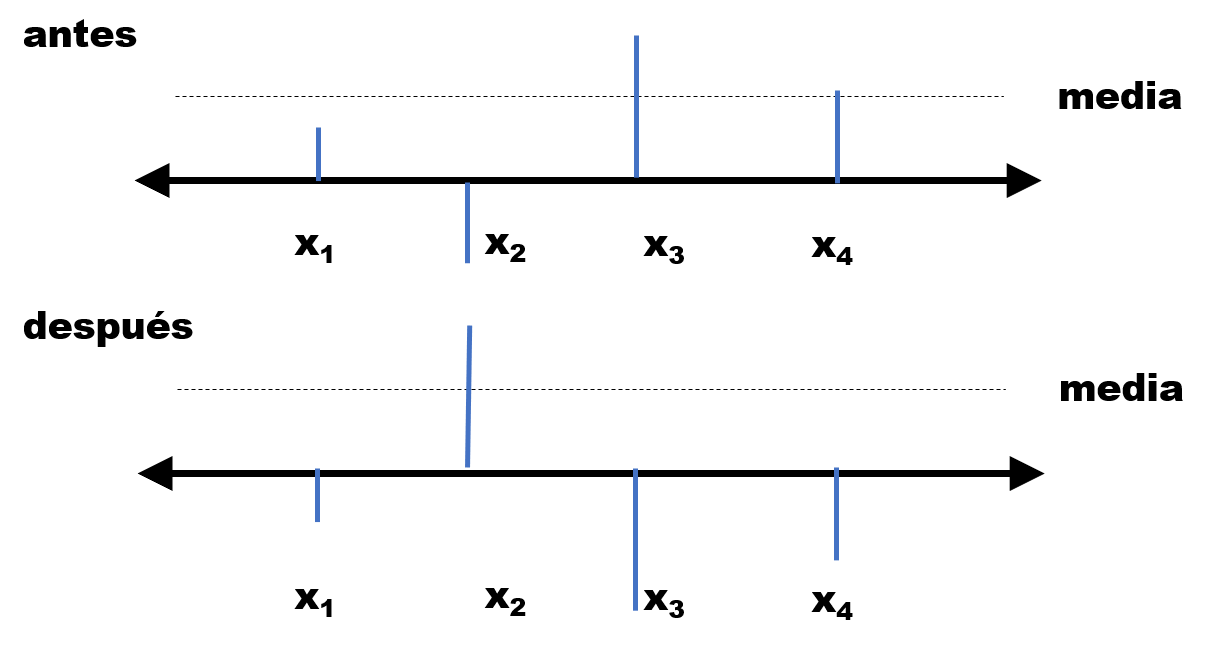
\includegraphics[scale=0.4]{figuras/inversionmedia.png}}
	\caption[Inversión sobre la media del algoritmo de Grover]{Inversión sobre la media del algoritmo de Grover. El conjunto de ${x_i}$ son las amplitudes de cada estado cuántico. La línea discontinua es la media de las amplitudes. Después de cada inversión, la amplitudes grandes se vuelven más grandes y las pequeñas más pequeñas. Fuente: elaboración propia}
	\label{fig:inversionmedia}
\end{figure}

En la Figura \ref{fig:inversionmedia} vemos que es una figura de elaboración propia, mientras que la Figura \ref{fig:distprob}, la fuente es un artículo cuya referencia viene indicada y el artículo es incluído en la Bibliografía.

\begin{figure}[h]
	\centerline{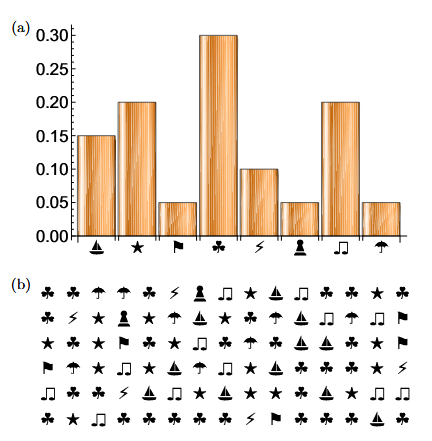
\includegraphics[scale=0.6]{figuras/distribucionprobabilidades.png}}
	\caption[Distribución de probabilidades]{a) Un ejemplo de distribución de probabilidad sobre 8 símbolos. (b) 100 muestras aleatorias de la distribución de probabilidad.
		probabilidad. El objetivo de un problema de muestreo es calcular muestras como las secuencias mostradas en (b) cuya complejidad	puede ser diferente a la complejidad de calcular la distribución de probabilidad (a). Fuente: \cite{lund2017}}
	\label{fig:distprob}
\end{figure}

\chapter{Discusión y conclusiones}

Las conclusiones es otra parte muy IMPORTANTE de la memoria. Deben ser muy claras. Si es posible se pueden itemizar o, mejor, poner un párrafo por idea con un pequeño título ilustrativo. En cualquier caso debe incluir los logros conseguidos y la importancia de los mismos, siempre desde un punto de vista crítico y resaltando las partes importantes.\\

\vspace{2cm}
{\bf{SOBRE LA EXTENSIÓN DEL TRABAJO}}\\

El Trabajo debe tener una extensión de 12$\pm$1 páginas. Los trabajos que no cumplan esta condición NO SE ACEPTARÁN. Las páginas que cuentan son las que van de la Introducción hasta estas Conclusiones. NO CUENTAN aquellas dedicadas a apéndices o a la Bibliografía.


\begin{thebibliography}{a}
	
%%\bibitem{etiqueta} \textsc{Autores},\textit{nombre referencia.}Información addicional

\bibitem[Aristóteles(trad. en 1995)]{aristóteles1995} Aristóteles (1995). \emph{Física} (Libro III, Capítulo 5, 1era ed. Guillermo R. de Echandía, trad.), Gredos.(Trabajo original publicado siglo IV A.C.)

\bibitem[Des-Cartes(1644)]{descartes1644} Des-Cartes, R. (1644). \emph{Principia philosophiae. En Zenodo (CERN European Organization for Nuclear Research)}, https://doi.org/10.5281/zenodo.7161988

\bibitem[Galileo(1632)]{galileo1632} Galilei, G. (1632). \emph{Dialogo di Galileo Galilei Linceo matematico sopraordinario dello studio di Pisa. E filosofo, e matematico primario del serenissimo gr. duca di Toscana. Doue ne i congressi di quattro giornate si discorre sopra i due massimi sistemi del mondo tolemaico, e.}, https://doi.org/10.5479/sil.77185.39088015628373

\bibitem[Gross(1996)]{gross1996} Gross, D. J. (1996). The role of symmetry in fundamental physics. \emph{Proceedings Of The National Academy Of Sciences, 93}(25), 14256-14259. https://doi.org/10.1073/pnas.93.25.14256

 \bibitem[Newton(2018)]{newton2018} Newton, I. (2018). \emph{Philosophiæ naturalis principia mathematica}, [HKUST Library], https://doi.org/10.14711/spcol/b706487
 
\bibitem[Noether(1918)]{noether1918} Noether, E. (1918). Invariante Variationsprobleme. \emph{Nachrichten von der Gesellschaft der Wissenschaften zu Göttingen, Mathematisch-Physikalische Klasse}, 235–257. https://eudml.org/doc/59024


 
%\bibitem[Lamport(1994)]{lamport1994} Lamport, L. (1994) \emph{\LaTeX: a document preparation system}, Addison Wesley, Massachusetts, 2nd ed.

%\bibitem[Ackerman(2017)]{ackerman2017} Ackerman, E. (2017) Why the English Premier League Should Have Playoffs.  Balls.ie. 

%\bibitem[Lund(2017)]{lund2017} Lund, A. P. and Bremner, Michael J. and Ralph, T. C. (2017) Quantum sampling problems, BosonSampling and quantum supremacy, npj Quantum Information 3: 15

\vspace{3cm}
Aún a riesgo de ser redundante, repito aquí que para consultar detenidamente la formas de referenciar, debéis seguir el formato APA del siguiente documento: \url{https://bibliografiaycitas.unir.net/documentos/APA_7ed_UNIR.pdf}

\end{thebibliography}

%\bibliographystyle{plain} 
%\bibliography{bibliografia}

\appendix
\chapter{Apéndices}

Aquí se pueden poner desarrollos matemáticos engorrosos de los que se puede prescindir en el cuerpo principal de la memoria u otros añadidos que aportan información pero no encajan correctamente en las secciones anteriores.

\end{document}

